%-*- coding: utf-8 -*-
%\input testHeada4
\documentclass[a4j,12pt]{jreport}
\newif\ifHMSol
\input macros.tex
\setlength{\textheight}{25.5cm}
\setlength{\textwidth}{0.8\paperwidth}
\setlength{\topmargin}{-1.3cm}
\setlength{\oddsidemargin}{0pt}
\setlength{\evensidemargin}{0pt}
%\setlength{\headheight}{0pt}
%\setlength{\headsep}{0pt}
%\setlength{\topskip}{0pt}
%\setlength{\footskip}{0pt}
%\pagestyle{empty}
%\input PrMacro
\newcommand{\SetTitleH}[5]{%
        \begin{center}
        {\Large #1 年度 #2 #3期試験問題(#4)}\\
                #5\\[-1em]
        \end{center}
%\vspace{0.5cm}\ 
}
\newcommand{\SetTitle}[5]{%
        \begin{center}
        {\Large #1 年度#2 #3 試験問題(#4)}\\% [-2.0em]
\setlength{\arrayrulewidth}{0.002\paperwidth}\setlength{\tabcolsep}{0mm}
  \begin{tabular}[t]{|*{2}{p{0.175\paperwidth}|}%
                      p{0.22\paperwidth}|p{0.11\paperwidth}|}
  \hline
  %\wellspaceside{科目名}&
  \wellspaceside{{学科$\bullet$組}}&
  \wellspaceside{学籍番号} &
  \wellspaceside{氏名} & \wellspaceside{採点}\\ \hline
  \rule{0mm}{0.033\paperheight}&  & & \\ \hline
  \end{tabular}\\[1em]
 {\bfseries 注意事項}
       \end{center}
 \begin{itemize}
 #5
\end{itemize} 
\vfill
\begin{center}
\setlength{\arrayrulewidth}{0.002\paperwidth}\setlength{\tabcolsep}{0mm}
\begin{tabular}{|*{5}{c|}}
\hline
\makebox[5em]{1} & \makebox[5em]{2} & \makebox[5em]{3} &
\makebox[5em]{4} & \makebox[5em]{5}\\\hline
 \rule[-2em]{0em}{4em}&&&&\\ \hline
\end{tabular}
\end{center}
\newpage
%\vspace{#5cm}\ 
}
%
\newcommand{\FBox}[1]{%
  \setlength{\fboxrule}{1pt}\fbox{\parbox{2.5em}{\small
  #1\rule[-1em]{0em}{1em}}} }
\newcommand{\StateTableN}[3]{%
\begin{center}%\Large
\begin{tabular}{|c|c|c|c|}
\hline
\smash{\raisebox{-0.8em}{状態}}& \multicolumn{2}{c|}{入力}&
\smash{\raisebox{-0.8em}{適格状態}}\\
\cline{2-3}
& \makebox[3em]{#1} &  \makebox[3em]{#2}&\\\hline
#3\\\hline
\end{tabular}\end{center}\rule{0em}{0em}
}
\newcounter{No}
\newcommand{\ShowNo}{
(\arabic{No})\stepcounter{No}&
(\arabic{No})\stepcounter{No}&
(\arabic{No})\stepcounter{No}&
(\arabic{No})\stepcounter{No}\\ \hline
   \makebox[3.5cm]{\rule{0cm}{2cm}}&
   \makebox[3.5cm]{\rule{0cm}{1cm}}&
   \makebox[3.5cm]{\rule{0cm}{1cm}}&
   \makebox[3.5cm]{\rule{0cm}{1cm}} \\ \hline
}
\newcommand{\ShowNoiii}{
(\arabic{No})\stepcounter{No}&
(\arabic{No})\stepcounter{No}&
(\arabic{No})\stepcounter{No}\\ \cline{1-3}
   \makebox[3.5cm]{\rule{0cm}{2cm}}&
   \makebox[3.5cm]{\rule{0cm}{1cm}}&
   \makebox[3.5cm]{\rule{0cm}{1cm}} \\ \cline{1-3}
}
\newcommand{\ShowNoii}{
(\arabic{No})\stepcounter{No}&
(\arabic{No})\stepcounter{No}\\ \cline{1-2}
   \makebox[3.5cm]{\rule{0cm}{2cm}}&
   \makebox[3.5cm]{\rule{0cm}{1cm}} \\ \cline{1-2}
}
\begin{document}
\SetTitle{2015}{後期}{ソフトウェア開発}{平野}
{\item 参照は配布資料、書籍が可能である。
\item {\bfseries パソコンは使用できない}。
\item 問題は1から\ref{lastProb}まであり、問題用紙はこの表紙を含めて\pageref{lastPage}枚ある。
試験開始直後に枚数に不足がないかどうか確認し、不足がある場合は直ちに申し出ること、
\item 解答は指定された解答欄に記入すること。}
\begin{Prob}\upshape
 次のHTMLファイルを実行したとき、コンソールにおける出力を記述しなさい。
 エラーが起こる場合はその旨、記述すること。
 {\small
 \listinginput{2}{t.html}
 }
\setcounter{No}{1}
\begin{center}
  \begin{tabular}{|c|c|c|c|}\hline
\ShowNo
\ShowNo
\ShowNo
\ShowNo
\ShowNoiii
 \end{tabular}
\end{center}\newpage
\end{Prob}
\begin{Prob}\upshape
 次のPHPファイルをコマンドプロンプトで実行したとき、その出力を記述しなさい。
 エラーが起こる場合はその旨、記述すること。
 {\small
 \listinginput{1}{t.php}
 }
\setcounter{No}{1}
\begin{center}
  \begin{tabular}{|c|c|c|c|}\hline
\ShowNo
\ShowNo
\ShowNo
\ShowNoii
 \end{tabular}
\end{center}\newpage
\end{Prob}
\begin{Prob}\upshape
  図\ref{css1}は\texttt{<div>}要素とスタイルシートを用いて表したものであ
 る。
 \begin{figure}[htb]
  \begin{center}
 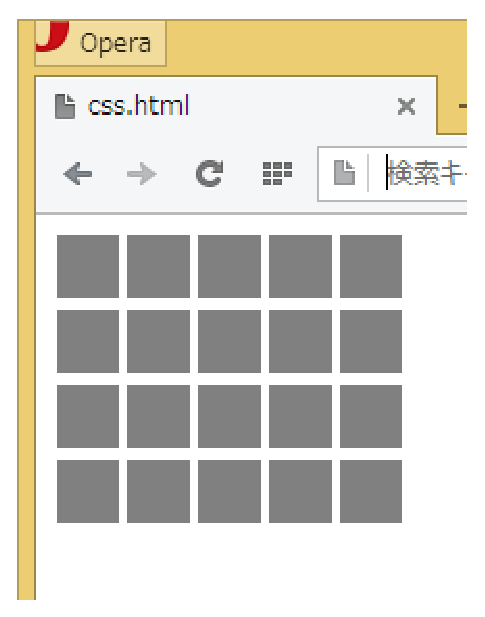
\includegraphics[width=3cm]{css1.eps}
  \end{center}
 \caption{基本のHTML文書の表示}\label{css1}
 \end{figure}

 この図のHTML文書のコードは次の通りである。
  {\footnotesize
 \listinginput{1}{css.html}}
 図\ref{css2},\ref{css3},\ref{css4}のようになるようにCSSセレクタを作成し
 なさい。縦横の\texttt{<div>}要素の数を変えても同様の結果になるのが望ま
 しい。なお、\verb+{background:yellow;}+の部分は必要ない。\\
\begin{minipage}{0.3\textwidth}
\begin{center}
 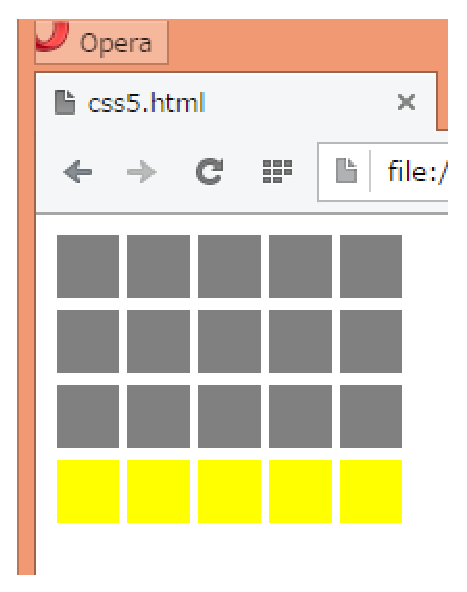
\includegraphics[width=3cm]{css5.eps}\\
\refstepcounter{figure} 図\thefigure : {一番下の横方向を黄色}\label{css2}
\end{center}     
 \end{minipage}
\begin{minipage}{0.3\textwidth}
\begin{center}
 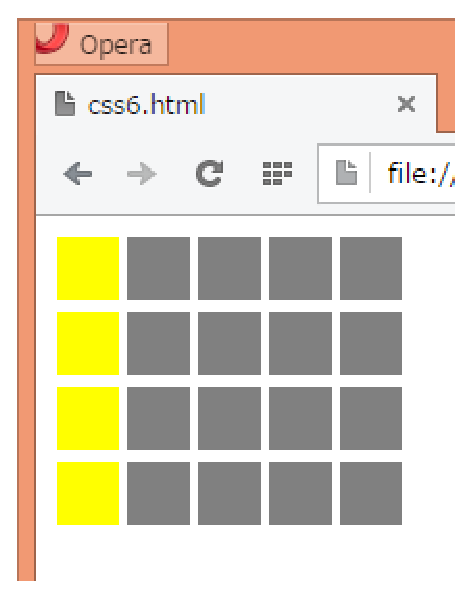
\includegraphics[width=3cm]{css6.eps}\\
\refstepcounter{figure} 図\thefigure : {一番左の縦方向を黄色}\label{css3}
\end{center}     
 \end{minipage}
\begin{minipage}{0.3\textwidth}
\begin{center}
 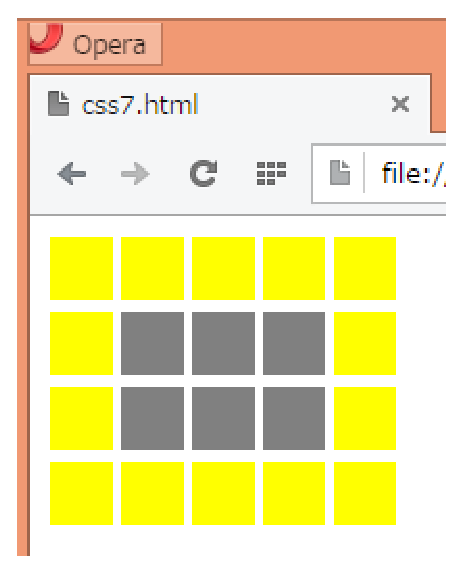
\includegraphics[width=3cm]{css7.eps}\\
\refstepcounter{figure} 図\thefigure : {一番外側を黄色}\label{css4}
\end{center}     
 \end{minipage}
\end{Prob}
\begin{center}
  \begin{tabular}{|c|c|c|}\hline
   図\ref{css2}&図\ref{css3} &図\ref{css4} \\\hline
   \makebox[5cm]{\rule{0cm}{3cm}}&
   \makebox[5cm]{\rule{0cm}{1cm}}&
   \makebox[5cm]{\rule{0cm}{1cm}} \\ \hline

 \end{tabular}
\end{center}
\newpage
 \begin{Prob}\upshape
次の関数\texttt{foo}の引数\texttt{x}と\texttt{y}は必須のもので、
\texttt{param1}と\texttt{param2}は関数内でデフォルト値が設定されており、
       必要に応じて変えることができる。
\begin{verbatim}
   function foo(x,y,param1,param2) {
     var def_param1 = 1, def_param2 ="default";
        ....
   }
\end{verbatim}
たとえば、\texttt{foo(x,y)}で呼び出されると\texttt{param1}と
       \texttt{param2}はそれぞれ\verb+def_param1+と\verb+def_param2+
       が使用される。

また、\texttt{foo(x,y,a)}で呼び出されると\texttt{param1}は\texttt{a}の値
       が、\texttt{param2}の値は\verb+def_param2+が使用される。

\texttt{param1}は\verb+def_param1+ を使用し、\texttt{param2}は与えられた
       値を使用するようにするためには関数の呼び出しはどのようにすればよ
  いか。また、引数の処理をするためにはど
  のようなコードを書けばよいか述べなさい。

  また、関数の仕様を変更して、\texttt{param1}などの引数をまとめてオブジェ
  クトで与え、与えられていない\texttt{param1}などの値はデフォルト値を設
  定するようにするにはどのようにすればよいか答えなさい。

 {\bfseries 解答欄}
 \end{Prob}\newpage
 \iffalse
   \begin{Prob}\upshape
    次のリストは有限集合を表すオブジェクトを作成している。
   {\small
    \listinginput{1}{prob.html}}
\begin{itemize}
 \item コンストラクタ関数で指定された要素を持つ数号のオブジェクトを作成
       する(8行目から34行目)。
 \item \texttt{Member} プロパティはその集合に属する要素の配列を返す。(14
       行目から22行目)
 \item \texttt{includes}メソッドは引数の要素がその集合に含まれているかど
       うかを判定する(23行目から24行目)。
 \item \texttt{includes}メソッドは引数の要素をその集合に追加する
       (25行目から32行目)。
 \item \verb+isEmpty()+メソッドは与えられた集合が空集合かどうか判定する
       (35行目)。
 \item \verb+foreach+メソッドは引数で与えられた関数を集合の各要素に適応
       する(37行目から39行目)。
 \item \verb+toString()+メソッドは文字列が必要な時にオブジェクトを文字列
       に変換する関数である(40行目から47行目)
\end{itemize}
 このプログラムを用いて、Operaのコンソールで動作させたところ次のように表
    示された。なお、\texttt{>}のついた行は入力した行であり、残りはブラウ
    ザからの出力である(一部改行している)。
    {\small
\begin{verbatim}
>A = new Set(1,2,3,4);
Set {length: 4, includes: function, add: function, Member: (...),
	isEmpty: function…}
>A+"";
"{1,2,3,4}"
A.add(1,5,6);
undefined
>A+"";
"{1,2,3,4,5,6}"
>A.Member;
["1", "2", "3", "4", "5", "6"]
>A.includes(10);
false
>A.includes(1);
true
>B = new Set();
Set {length: 0, includes: function, add: function, Member: (...),
	isEmpty: function…}
>B.isEmpty();
true
\end{verbatim}
}
次の問いに答えなさい。
\begin{enumerate}
 \item 10行目に現れる\texttt{arguments}変数について説明しなさい。\\[2cm]
 \item 40行目から48行目で定義されている\verb+toString()+メソッドで41行目の処
       理が必要な理由を述べなさい。\\[2cm]
 \item 9行目で宣言されている\verb+Member+と37行目で呼ばれている
       \verb+this.Member+ の違いについて説明しなさい。\\[2cm]
 \item \verb+add()+メソッドで既に存在している要素が二重に追加されない理
       由を説明しなさい。\\[3cm]
 \item このオブジェクトの不備な点について理由をつけて挙げなさい。
\end{enumerate}
 \end{Prob}\newpage
 \fi
\begin{Prob}\label{lastProb}
 \upshape
 次の項目のうち一つを選んで100文字以上で解答しなさい。
 \begin{itemize}
  \item JavaScriptの言語の特性について考察しなさい。
  \item jQuery では同じメソッドに対して引数の数で動作が異なる設計をしてい
	る。この点についてのメリット、デメリットに
	ついて論じなさい。また、jQueryライブラリーを使うメリット、デメリットに
	ついても論じなさい。
  \item Google Maps ではオブジェクトのパラメータをJavaScriptのオブジェク
	トリテラルの形式で与えているが、この方法もメリット、デメリットに
	ついて論じなさい。
  \item この授業で学んだことについて、重要と思われる点を取り上げ、その理
	由について述べなさい。
 \end{itemize}
 {\bfseries 解答欄}
\end{Prob}
\label{lastPage}
\end{document}